\documentclass[10pt, conference, compsocconf]{IEEEtran}
\usepackage{xltxtra}
\usepackage{subfig}
\usepackage{booktabs}
\usepackage{amsmath}
\usepackage{flushend}
\usepackage[numbers,sort&compress]{natbib}
\setmainfont{Times New Roman}

\begin{document}

\title{igrow: A Multithreaded Ligand Synthesis Tool for Structure-Based Molecular Design} % can use linebreaks \\ within to get better formatting as desired
\author
{
\IEEEauthorblockN
{
Hongjian Li\IEEEauthorrefmark{1}, Ching-Man Tse\IEEEauthorrefmark{1}, Kwong-Sak Leung\IEEEauthorrefmark{1}, Man-Hon Wong\IEEEauthorrefmark{1}, Kin-Hong Lee\IEEEauthorrefmark{1} and Mary Miu-Yee Waye\IEEEauthorrefmark{2}
\IEEEauthorblockA
{
\IEEEauthorrefmark{1}
Department of Computer Science and Engineering, Chinese University of Hong Kong, Hong Kong, P.R. China\\
\{hiji, cmtse, ksleung, mhwong, khlee\}@cse.cuhk.edu.hk
}
\IEEEauthorblockA
{
\IEEEauthorrefmark{2}
School of Biomedical Sciences, Chinese University of Hong Kong, Hong Kong, P.R. China\\
mary-waye@cuhk.edu.hk
}
}
}
\maketitle

\begin{abstract}



\end{abstract}

\begin{IEEEkeywords}

bioinformatics, chemoinformatics, drug discovery, molecular docking, virtual screening, ligand synthesis, molecular design, multithreading

\end{IEEEkeywords}

\section{Introduction}

Fragment linking method exxample \citep{An Ab Initio Method for Designing Multi-Target Specific Pharmacophores using Complementary Interaction Field of Aspartic Proteases}
Properitary software \citep{Incorporating Virtual Reactions into a Logic-Based Ligand-Based Virtual Screening Method to Discover New Leads}

As the X-ray crystallography technology evolves, more and more structures of biological macromolecules at atomic level have been revealed and deposited into the world's largest repository Protein Data Bank (PDB) \cite{539,537}. This rapid evolution catalyzes the development of various protein-ligand docking tools for structure-based drug discovery.

Protein-ligand docking is a method which predicts the preferred conformation of a small ligand when bound to a macro protein to form a stable complex. It also predicts the binding affinity in terms of free energy, which is basically the overall effect of various chemical forces involved. The lower the free energy, the higher the binding affinity. Very often, the target protein is a viral enzyme of interest, and the small organic ligands that are predicted to inhibit the viral enzyme are what we want to discover. Structure-based virtual screening is simply a massive version of docking. It docks a database of drug-like ligands to a target, ranks them according to their predicted binding affinity, and shortlists the best ones for further investigation.

\textit{De novo} ligand design and protein-ligand docking are closely related. Tiny fragments are combined in accordance to chemistry rules to synthesize larger ligands, which are then docked to a receptor to evaluate their fitness. The best ligands enter the next iteration to synthesize other ligands, which are again evaluated by docking, until promising ligands are discovered. AutoGrow \citep{466}, released in \citeyear{466}, is a representative \textit{de novo} ligand design tool that makes use of genetic algorithm and AutoDock Vina \citep{595} to automate this recursive synthesis/docking procedure.

In 2011, inspired by AutoGrow, we developed SmartGrow, addressing several problems that AutoGrow suffers from. SmartGrow not only inherited the selection, mutation and crossover operators from AutoGrow, but also invented our novel merge and split operators. It implemented Lipinski's \textit{Rule of Five} \citep{168} to ensure drug likeness. Its robust parser correctly processed two-letter chemical elements like Cl (chlorine) and Br (bromine), and meanwhile added additional support for P (phosphorus), a common chemical element found in many drugs. Results showed that SmartGrow displayed comparable performance in terms of predicted free energy and meanwhile outperformed AutoGrow by 30\% in terms of execution time on average across 18 test cases. Besides, ligands generated by SmartGrow resulted in 100g/mol lower molecular weights than AutoGrow and never exceeded 500g/mol so that they can be absorbed by human body.

However, we wrote SmartGrow in a hurry and did not follow a formal software engineering approach. Later on when we conducted a benchmark on SmartGrow, we discovered a great many of exceptional bugs that were rather hard to track due to the messy code structure and lack of comments. Regretfully, we decided to abandon our buggy SmartGrow.

\section{Motivation}



\section{Methods}

Figure \ref{fig:Flowchart} shows the overall flowchart of igrow. 

\begin{figure}
\centering
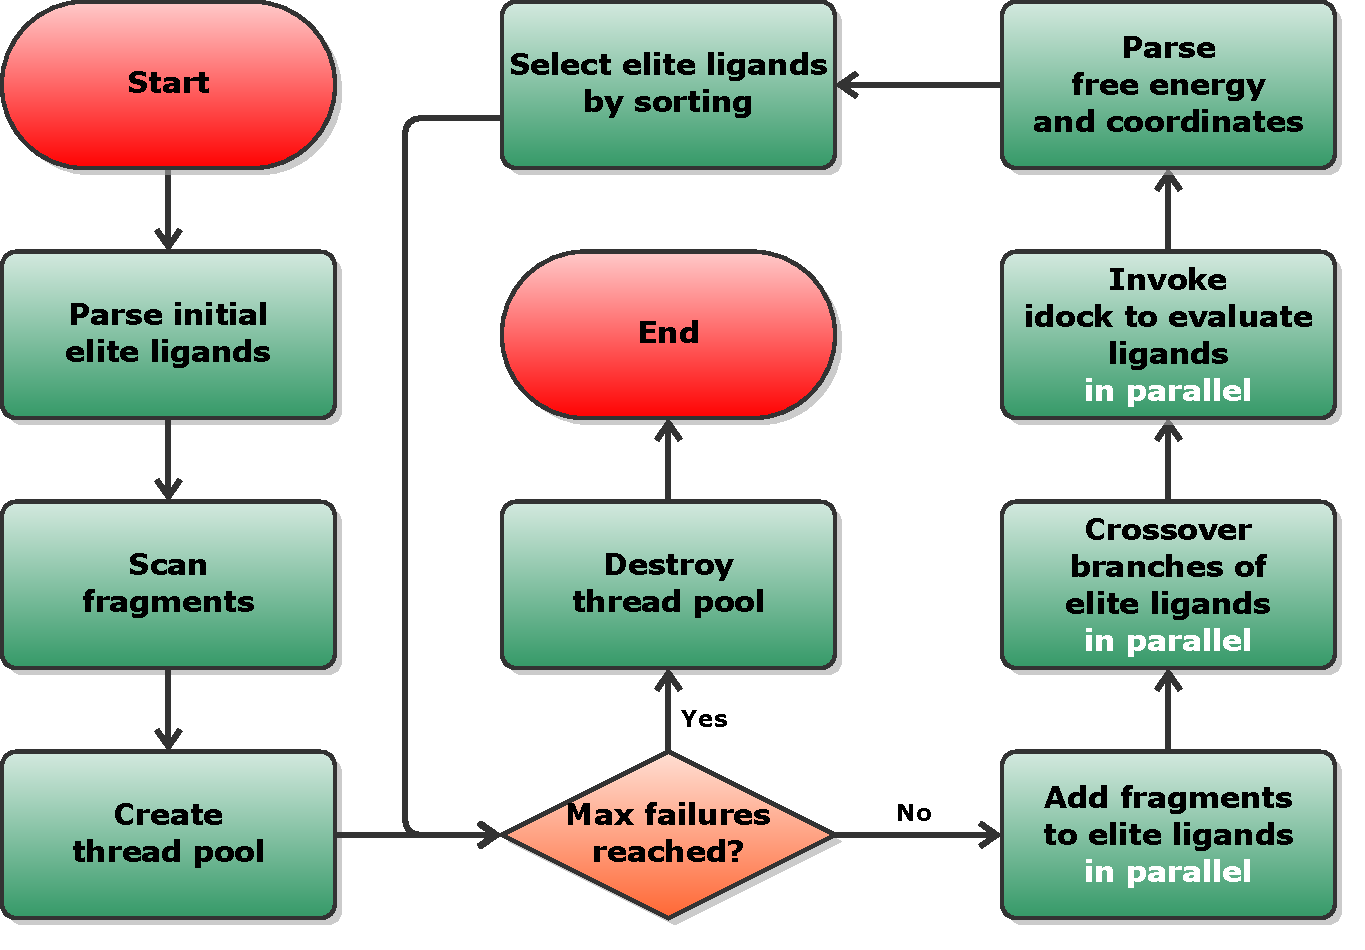
\includegraphics[width=\linewidth]{../igrow/Flowchart.pdf}
\caption{Flowchart of igrow.}
\label{fig:Flowchart}
\end{figure}

igrow remarkably revises the fundamental C++ implementation. igrow invents its own thread pool in order to reuse threads and maintain a high CPU utilization throughout the entire screening procedure. The thread pool parallelizes the execution of mutation and crossover operators. igrow estimates the capacity of every vector structure and intensively utilizes Rvalue reference, a new feature in the C++11 standard, to avoid frequent memory reallocation. igrow accelerates the assignment of atom types by making use of residue information for receptor and branch information for ligand, without explicitly detecting covalent bonds among atoms.
We then developed igrow as a successor of SmartGrow. Instead of porting existing code from SmartGrow and fixing bugs line by line, we rewrote igrow from scratch in a systematic manner. We borrowed several great ideas from idock, and deliberately designed igrow in the way that the output of idock directly feeds igrow as its input. Figure \ref{igrow:Flowchart} shows the flowchart of our current implementation of igrow. During initialization, igrow parses the initial elite ligands predicted by idock in a previous run, and scans a user-specified folder for fragments. Likewise in idock, igrow also creates a novel thread pool in order to parallelize the genetic operators and reuse threads throughout the entire synthesis procedure. Then igrow enters a loop, and utilizes genetic algorithm to iteratively synthesize novel ligands in parallel by either addition, subtraction or crossover, and invoke idock externally to predict free energy and select elite ligands by sorting the predicted free energy asendingly. So far we have completed the program, and are now fixing bugs and evaluating it.

\begin{figure}
\centering
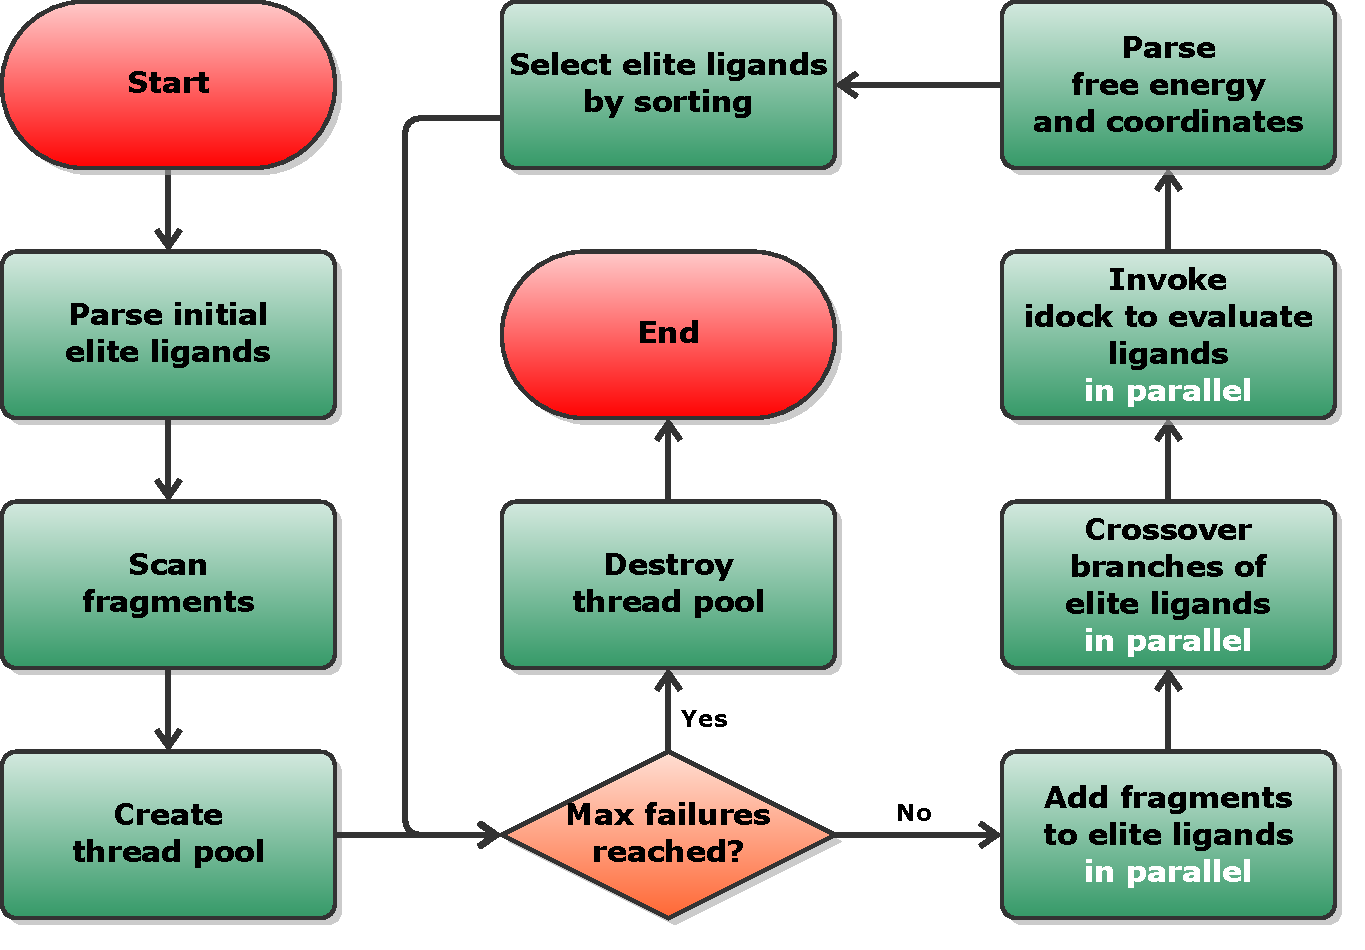
\includegraphics[width=\textwidth]{../igrow/Flowchart.pdf}
\caption{igrow flowchart.}
\label{igrow:Flowchart}
\end{figure}

Figure \ref{igrow:Addition} illustrates the addition operator in igrow. An elite ligand and a fragment are randomly selected and merged by removing a hydrogen atom from both sides and forming a new rotatable bond to connect both sides, thereby constructing an elite ligand. The addition operator may produce novel ligands that display a higher binding affinity but may also suffer from a larger molecular weight. Figure \ref{igrow:AdditionComplex} draws the three elitsts in complex with their target protein. Due to the presence of additional fragments, the elite ligands may occupy significantly different binding conformations.

\begin{figure}
\centering
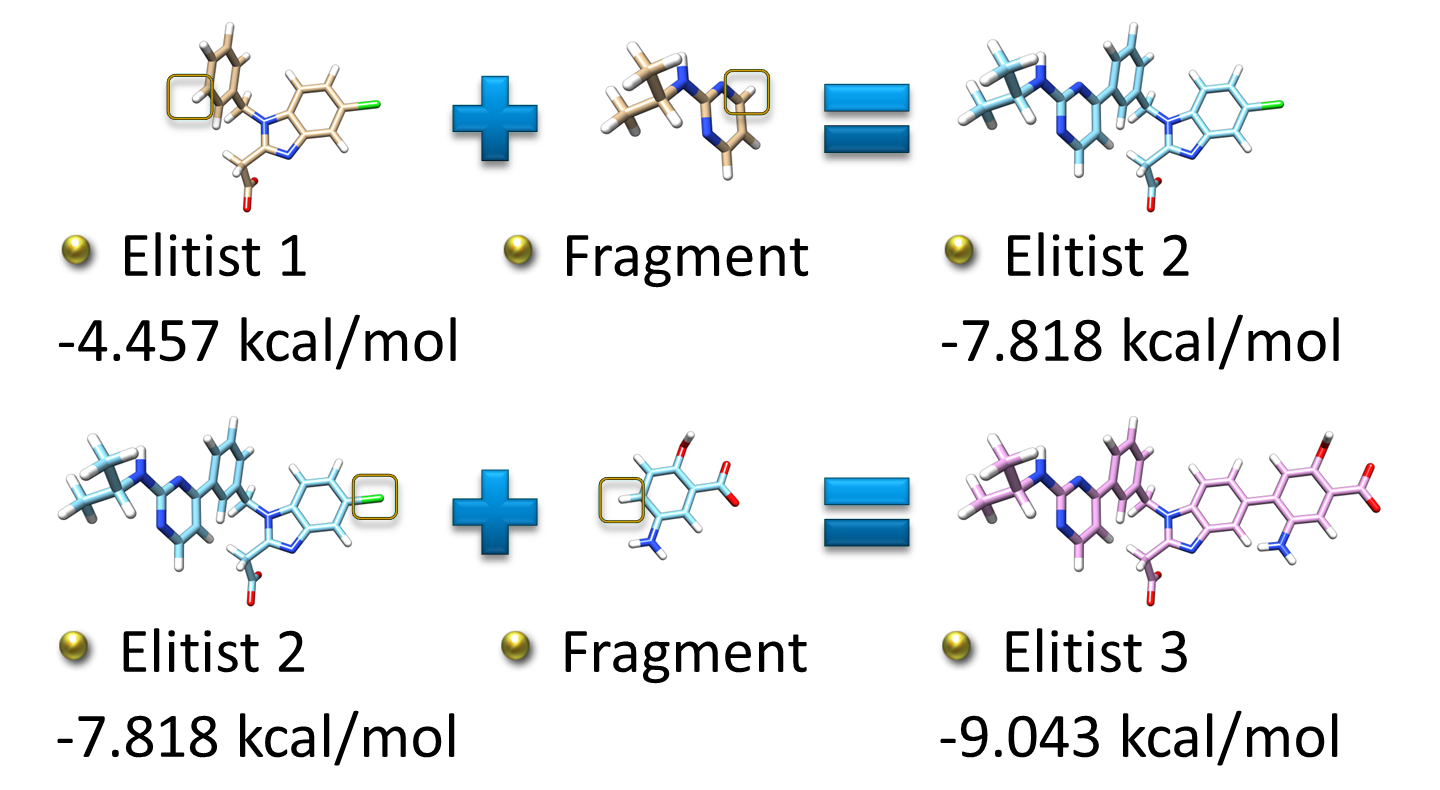
\includegraphics[width=\textwidth]{../igrow/Addition.png}
\caption{igrow addition operator.}
\label{igrow:Addition}
\end{figure}

\begin{figure}
\centering
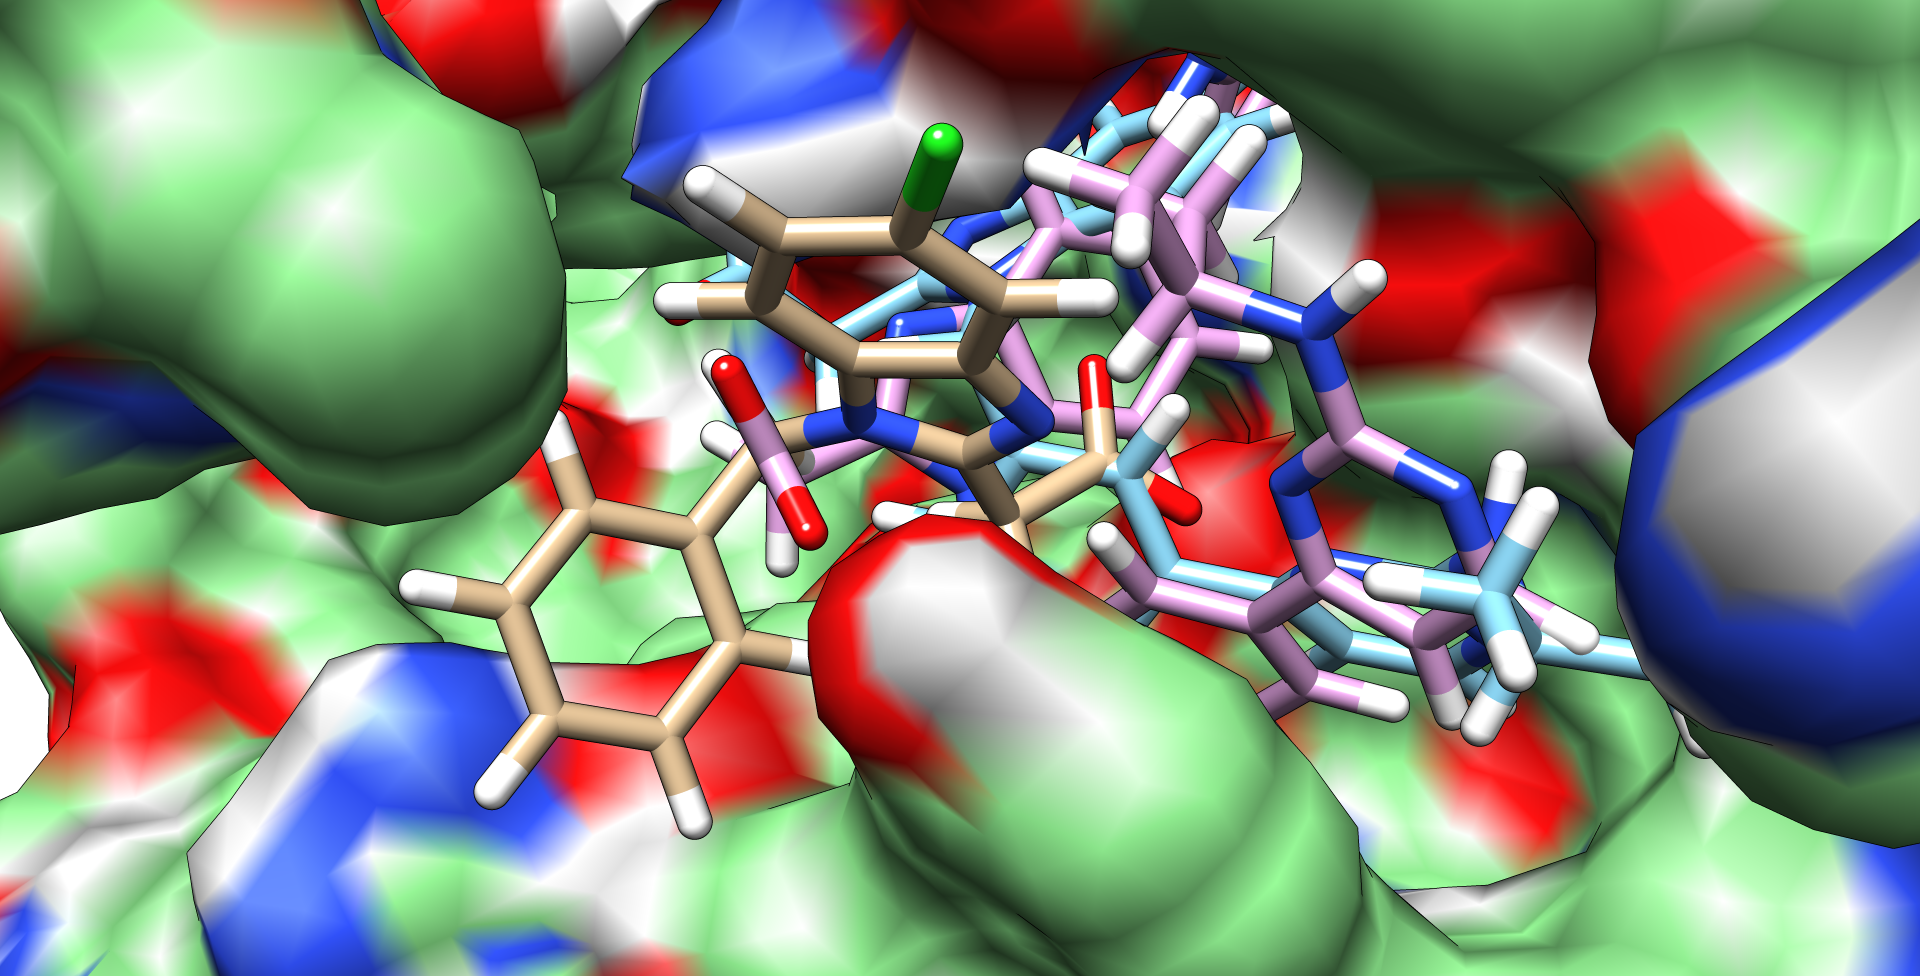
\includegraphics[width=\textwidth]{../igrow/AdditionComplex.png}
\caption{Synthesized elitists by addition in complex with their target protein.}
\label{igrow:AdditionComplex}
\end{figure}

Figure \ref{igrow:Subtraction} illustrates the subtraction operator in igrow. An elite ligand and one of its rotatable bonds are randomly selected. The ligand is split into two by breaking the rotatable bond and substituting a hydrogen, thereby constructing a smaller ligand. The subtraction operator may produce novel ligands that display a lower binding affinity but may also benefit from a smaller molecular weight.

\begin{figure}
\centering
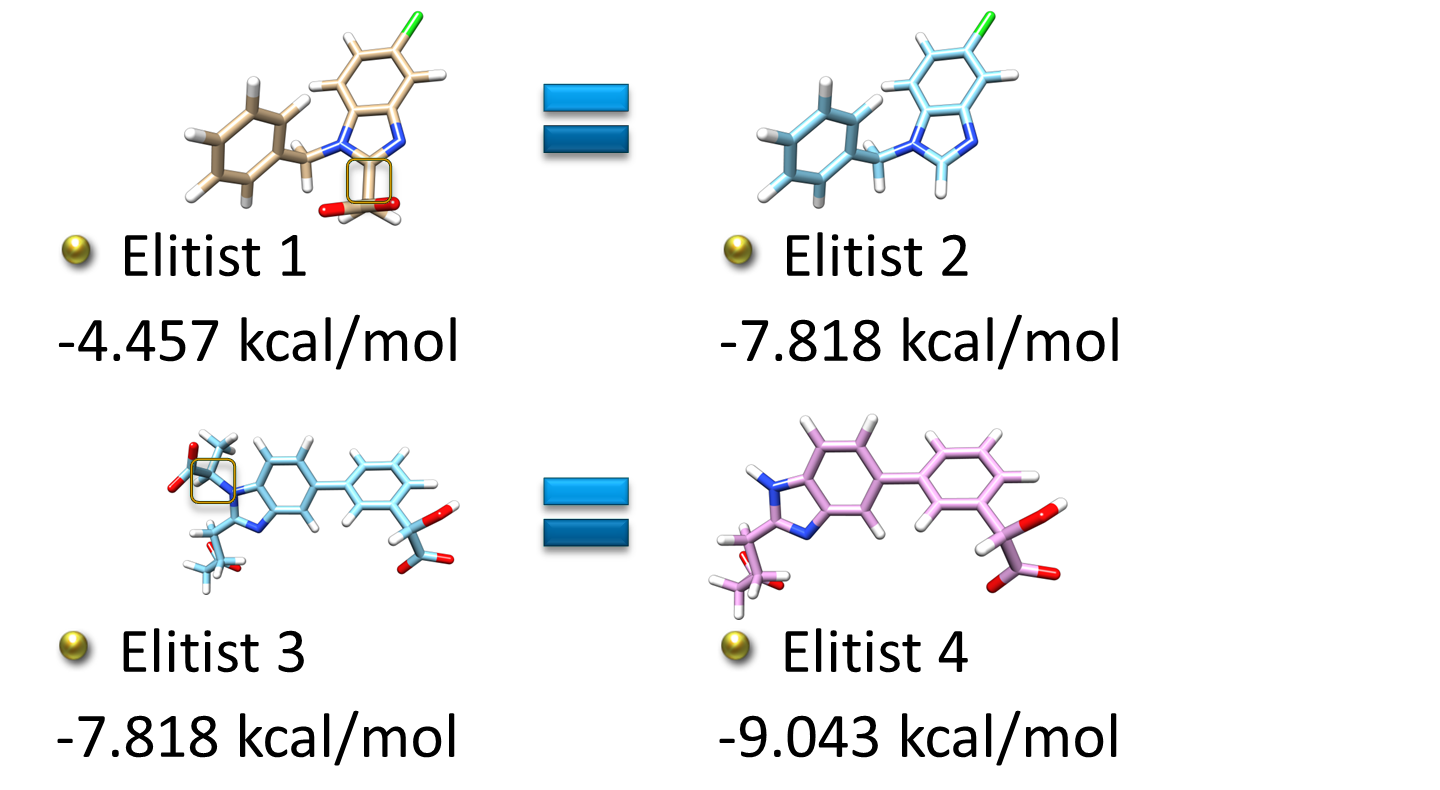
\includegraphics[width=\textwidth]{../igrow/Subtraction.png}
\caption{igrow subtraction operator.}
\label{igrow:Subtraction}
\end{figure}

Figure \ref{igrow:Crossover} illustrates the crossover operator in igrow. Two elite ligands are randomly selected and parts of them are exchanged, thereby constructing an elite ligand. The crossover operator may produce novel ligands that display either a higher binding affinity or a lower binding affinity. Figure \ref{igrow:CrossoverComplex} draws the three elitsts in complex with their target protein. Due to the exchange of molecular moieties, the elite ligands may occupy significantly different binding conformations.

\begin{figure}
\centering
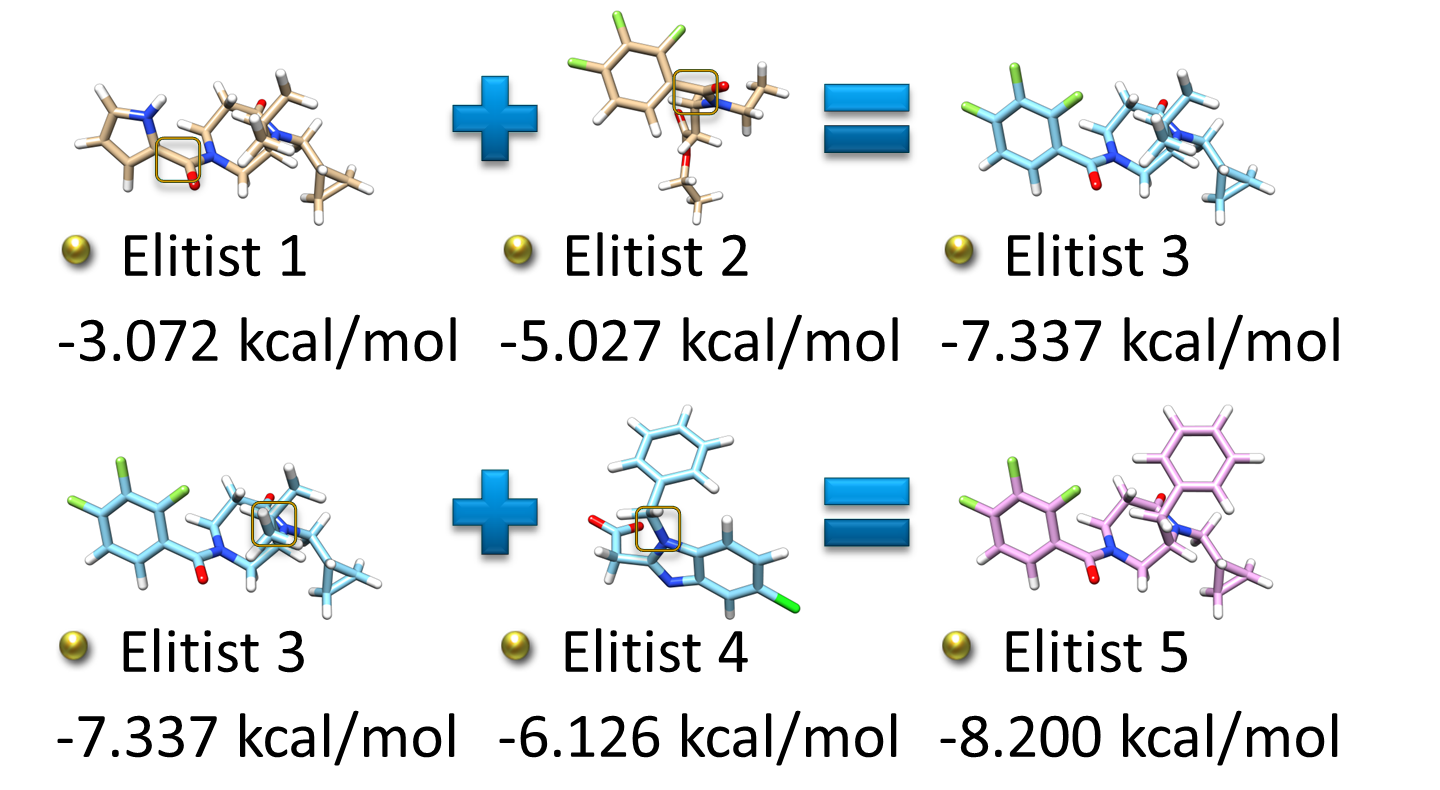
\includegraphics[width=\textwidth]{../igrow/Crossover.png}
\caption{igrow crossover operator.}
\label{igrow:Crossover}
\end{figure}

\begin{figure}
\centering
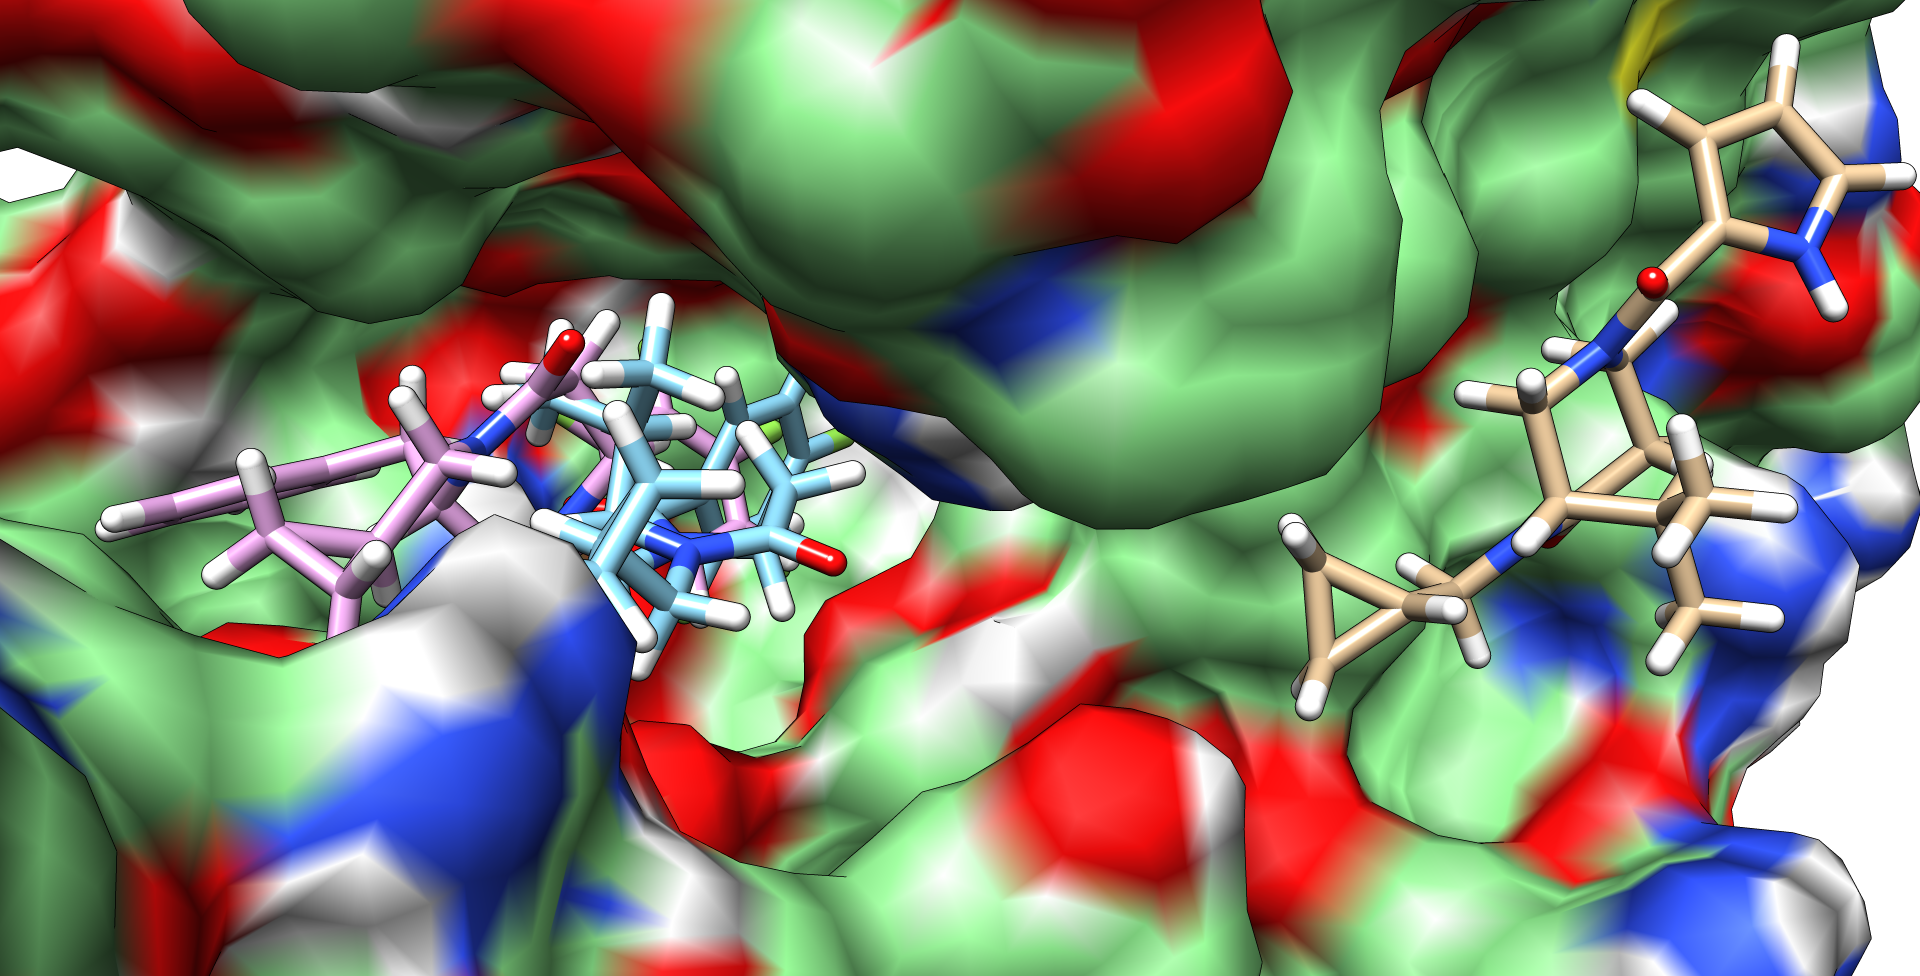
\includegraphics[width=\textwidth]{../igrow/CrossoverComplex.png}
\caption{Synthesized elitists by crossover in complex with their target protein.}
\label{igrow:CrossoverComplex}
\end{figure}

\section{Data}

In order to test igrow comprehensively, we collected 3 receptors from PDB \cite{96} and 8 unique initial ligands from PDB and ZINC \cite{55}. From these data, 18 test cases could be formed, as detailed below.

\subsection{Receptors}

We aim to select receptors that are of real-life importance. Glycogen synthase kinase 3 beta (GSK3$\beta$) is a theoretically promising pharmacotherapeutic target for the treatment of several human diseases, including type-2 diabetes \cite{247} and Alzheimer's disease (AD) \cite{248}. Efforts into discovering new inhibitors of GSK3$\beta$ never stop \cite{246}. Therefore it was included into our test data.

HIV was also selected for its impact to human kind. According to the latest fact sheets of World Health Organization in 2010, 33.4 million people live with HIV/AIDS worldwide. HIV reverse transcriptase (HIV RT) and HIV protease (HIV PR), two viral proteins residing in the body of the virus, assist the virus in infecting human cells. Researchers have spent over 30 years in discovering new inhibitors of HIV RT and HIV PR \cite{221,222,223}. Therefore, they were also included into our test data.

Totally 3 receptors were collected from PDB \cite{96} for testing. They are glycogen synthase kinase 3 beta (GSK3$\beta$) of PDB ID 1J1B \cite{245} of resolution 1.80 \AA, HIV reverse transcriptase (HIV RT) of PDB ID 2ZD1 \cite{180} of resolution 1.80 \AA, and HIV protease (HIV PR) of PDB ID 3KFN \cite{243} of resolution 1.77 \AA.

We manually extracted the 3 receptors out of their PDB complexes, and queried CSA (Catalytic Site Altas) \cite{206} and relevant publications \cite{245,246,180,221,222,223,243} for their possible binding sites, as shown in table \ref{tab:searchspace}.

\begin{table*}
\centering
\begin{tabular*}
{\linewidth}
{@{\extracolsep{\fill}}lccc}
\noalign{\smallskip}
\toprule
Receptor & Glycogen synthase kinase 3 beta & HIV reverse transcriptase & HIV protease\\
\midrule
\noalign{\smallskip}
PDB ID & 1J1B & 2ZD1 & 3KFN\\
Resolution & 1.80 \AA & 1.80 \AA & 1.77 \AA\\
Selected binding site & Catalytic site & Allosteric site for NNRTI binding & Exo site\\
Grid box center & (20.304 \AA, 16.365 \AA, -9.814 \AA) & (49.712 \AA, -28.441 \AA, 35.555 \AA) & (8.113 \AA, 9.701 \AA, 4.310 \AA) \\
Grid box size & 22 x 18 x 20 \AA$^3$ & 16 x 16 x 18 \AA$^3$ & 22 x 26 x 22 \AA$^3$\\
\bottomrule
\end{tabular*}
\caption{PDB IDs, resolutions, selected binding sites, grid box centers and sizes of the 3 testing receptors. NNRTI stands for non-nucleotide reverse transcriptase inhibitor. The exo site of HIV protease refers to the exo site adjacent to the Gly$^{16}$Gly$^{17}$Gln$^{18}$ loop.}
\label{tab:searchspace}
\end{table*}

\subsection{Initial Ligands}

We aimed to select initial ligands that spread across wide ranges of free energies and molecular weights. The 3 ligands of PDB heterogeneous molecule IDs TRS, T27 and 4DX are respectively native ligands of GSK3$\beta$, HIV RT and HIV PR, hence they were included.

\subsection{Fragment Library}

ZINC clean shards

\section{Results}

We tested igrow v1.0 and compared it with AutoGrow 2.0.4, the most recent versions of both programs at the moment this paper was composed. The parameter settings for AutoGrow and igrow are listed in table \ref{tab:ParameterSettings}. The default values for AutoGrow were retained, i.e. 10, 20, 20, and 8 for the number of elitists, children, mutants, and generations, respectively.

\begin{table}
\centering
\begin{tabular*}
{\linewidth}
{@{\extracolsep{\fill}}lrr}
\noalign{\smallskip}\toprule
Program & AutoGrow & igrow\\
\midrule
\noalign{\smallskip}
Number of elitists & 10 & 10\\
Number of children & 20 & 20\\
Number of mutants & 20 & 20\\
Number of generations & 8 & 24\\
Max number of atoms & 80 & 80\\
\bottomrule
\end{tabular*}
\caption{Parameter settings for AutoGrow and igrow. Elitists refer to the best ligands of a generation that will survive directly into the next generation. Children refer to ligands generated by crossover. Mutants refer to ligands generated by mutation.}
\label{tab:ParameterSettings}
\end{table}

So far we have collected 3 receptors, each of which is associated with 6 initial ligands. Therefore there are 18 test cases in total. Since genetic algorithm is stochastic, we ran AutoGrow and igrow for 9 times for each test case under the parameter settings shown in \ref{tab:ParameterSettings}, simultaneously on 6 Linux machines with Ubuntu 10.04.1 x86\_64, Dual Intel Xeon Quad Core 2.4GHz, and 32GB RAM. Each AutoGrow execution and igrow execution cost approximately 3 hours and 2.4 hours respectively on average.

\subsection{Binding Pose}

In order to validate the correctness of ligands generated by igrow, we picked out the best ligand from each test case and visualized it in complex of its corresponding receptor. Here, the best ligand refers to the one that have the lowest free energy.
Figure \ref{fig:BestLigands} demonstrates one particular test case.

\subsection{Free Energy and Molecular Weight}

The goal of fragment-based growing strategy is not to generate one single best ligand, but a population of drug-like ligands to be shortlisted for further verifications by wet lab experiments. Therefore it is more meaningful to dig into the average performance of the best several ligands. Hence the predicted free energies and molecular weights of the best 5 ligands were plotted against generation number in figure \ref{fig:Best5}.

\subsection{Execution Time}

We also measured the execution times of AutoGrow and igrow. Since all the test cases were run for 9 times, their average execution times are shown in figure \ref{fig:ExecutionTime}.

\section{Discussions}

Through visualizing the generated ligands in complex of their respective receptors, we found that they are chemically valid, and we are thus of full confidence about the correctness of igrow. An example test case is demonstrated in figure \ref {fig:BestLigands}.
The best ligands generated by igrow have significantly lower molecular weights than those generated by AutoGrow, hence they are more likely to optimize into drugs.

Regarding the average free energies and molecular weights of the best 5 ligands generated by both programs, as shown in figure \ref{fig:Best5}, for most of the cases igrow displays a comparable free energy curve, while its molecular weight curve is remarkably lower than AutoGrow, and seldom exceeds 500, thanks to the guidance of Lipinski's rule of five and the `split' operator.

Regarding the execution time, as shown in figure \ref{fig:ExecutionTime}, igrow outperforms AutoGrow for 14 out of 18 test cases.
For the test case with GSK3$\beta$ as the receptor and ZINC20030231 as the initial ligand, igrow runs as much as 119\% faster than AutoGrow.
For the test case with HIV RT as the receptor and T27 as the initial ligand, although igrow requires 27\% more time, the generated ligands have lower free energies, as shown in figure \ref{fig:Best5}(g).
Averaging all the 18 test cases, in general igrow executes about 30\% faster than AutoGrow.

Compared to AutoGrow and SmartGrow, our igrow features a plenty of advantageous innovations. From the perspective of input and output, igrow supports direct PDBQT manipulation, i.e. it digests ligands and fragments in PDBQT format and outputs ligands also in PDBQT format, saving the effort of frequently calling external python script for format conversion. igrow utilizes flyweight programming pattern to cache fragments and dynamic pointer vector to cache and sort ligands. From the perspective of CPU and memory utilization, igrow inherits from idock the highly efficient thread pool to parallelize the two genetic operators and maintain a high CPU utilization. igrow estimates the capacity of every vector structure and intensively utilizes right value reference, a new feature in the C++11 standard, to avoid frequent memory reallocation. From the perspective of functional improvements, in addition, igrow supports halogen replacement as a new type of synthesis in addition to hydrogen replacement, in subtraction, igrow supports spliting a ligand into two by breaking a rotatable bond and substituting a hydrogen, and in crossover, igrow supports branch replacement, and in selection, igrow refreshes ligands with docked coordinates, potentially enabling partial docking as detailed below. igrow traces the sources of synthesized ligands and outputs statistics in CSV format for users to easily analyze how new ligands are synthesized from initial elite ligands and fragments (Figure \ref{igrow:SyntheticTraceability}). igrow allows users to specify ranges of several chemical properties, including molecular weight, number of atoms, number of heavy atoms, number of rotatable bonds, number of hydrogen bond donors and number of hydrogen bond acceptors, as validators for newly synthesized ligands. igrow is designed in a flexible way that it reserves room for adaptation to new molecular constraints. Instead of simply depending on the number of generations as a stopping criterion, igrow allows users to specify the number of validation failures as a more reasonable stopping criterion.

\begin{figure}
\centering
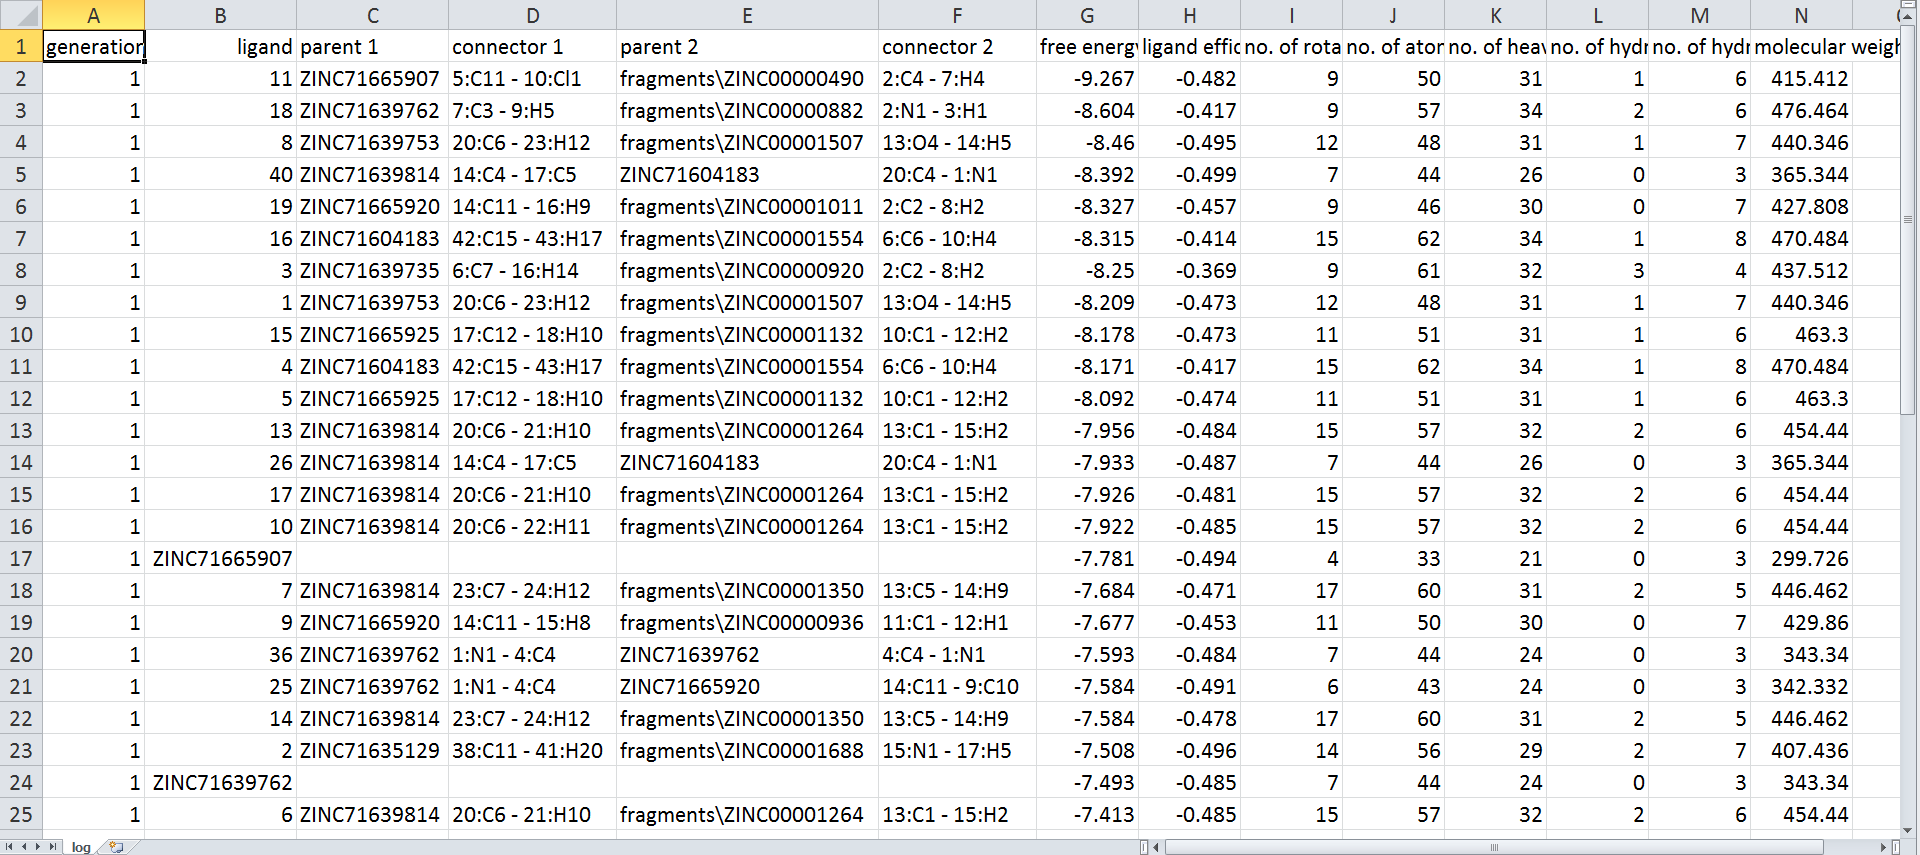
\includegraphics[width=\textwidth]{../igrow/SyntheticTraceability.png}
\caption{igrow synthetic traceability.}
\label{igrow:SyntheticTraceability}
\end{figure}

Clearly, there are two major problems with our current design. Problem one is the chemical infeasibility of ligands synthesized. This is a functional problem. Problem two is the high cost of invoking external idock in every generation. This is a computational problem.

Functionally speaking, ligands synthesized by our genetic operators, albeit chemically valid, might not be chemically synthesizable, simply because the two operators are somewhat arbitrary and do not conform to any known or general chemical reactions. In other words, that we can computationally synthesize novel ligands does not imply we can chemically synthesize them in reality. We may produce very fancy ligands at will, but all are just in computer simulation.

Computationally speaking, igrow relies on idock as its external docking engine and thus has to invoke idock every generation after synthesizing new ligands, repeatedly reading identical receptor and creating identical grid maps. Such duplications prolong program execution time quite a bit as the number of generations increases in genetic algorithm.

We propose idock 4.0 to address the above two problems. On one hand, inspired by AutoClickChem \citep{1051}, we plan to incorporate click chemistry into igrow to make sure every step of synthesis does follow some kind of well-known chemical reaction. On the other hand, we plan to integrate igrow into idock. In addition to receptor and grid map caching, another advantage of integration is the capability of partial docking, which refers to holding the main body of a ligand rigid while merely rotating newly added fragments. By cutting off the positional and orientational degrees of freedom, obviously partial docking can dramatically reduce search space dimensionality and therefore dramatically speed up the selection operator, which is the bottleneck of igrow.

\section{Availability}

As for software availability, igrow is free and open source under Apache License 2.0. It is written in C++ and available at https://github.com/HongjianLi/igrow. Precompiled executables for 32-bit and 64-bit Linux, Windows, Mac OS X, FreeBSD and Solaris are provided. Use cases and API documentations are also provided.

igrow is free and open source under Apache License 2.0. It is written in C++ and available at http://GitHub.com/HongjianLi/igrow. Precompiled executables for 32-bit and 64-bit Linux, Windows, Mac OS X, FreeBSD and Solaris are provided. Docking examples and API documentations are also provided.

\section{Conclusions}

We have developed igrow, an efficient tool for computational synthesis of potent ligands.

\bibliographystyle{unsrtnat}
\bibliography{refworks}

\end{document}
